\documentclass[]{report}
\usepackage{graphicx, float,}
\usepackage{hyperref}
\usepackage[export]{adjustbox}

\title{\centering CSP334 : Computer Networks \\Lab Assignment No 6\\Assignment on DNS}
\author{\LARGE Sahil\\2016UCS0008}

% to use proper section numbering in the report type 
\renewcommand{\thesection}{\arabic{section}}

\begin{document} 

\maketitle

%%%%%%%%%%%%%%%%%%%%%%%%%%%%%%%%%%%%%%%%%%%%%%%%
\section{SET 1: The Basic DNS:}

\subsection{:}
\large
The transport layer protocol used for sending the DNS queries is \textbf{UDP}.
\\
\textbf{Benefits of UDP:} There is no connection establishment in UDP, so there is no need to maintain connection state. Hence, it is a simple protocol. 
\\
Also, data is not retransmitted if there is any loss of data, which can be used in time sensitive applications like real-time audio or video. 
\\
\textbf{Drawbacks of UDP:} Data loss can occur as it does not provide reliability. Also, no timing and minimum throghput guarantees are provided.

\subsection{:}
\begin{figure}[H]
	\vspace{0pt}
	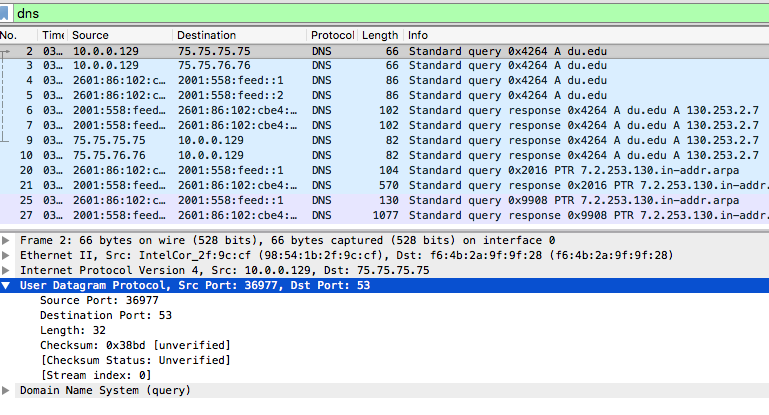
\includegraphics[height = 250pt, keepaspectratio]{Snapshots/q1/1_2.png}
\end{figure}

The port numbers used for sending the packet is $36977$ and receiving the packet is $53$. 

\subsection{:}
- The destination of packet $2$ is $75.75.75.75$. \\
- It is a DNS query of type \textbf{A} as shown. In this, we give the hostname in the query and receive the IPA in the response. 
\\
\begin{figure}[H]
	\vspace{0pt}
	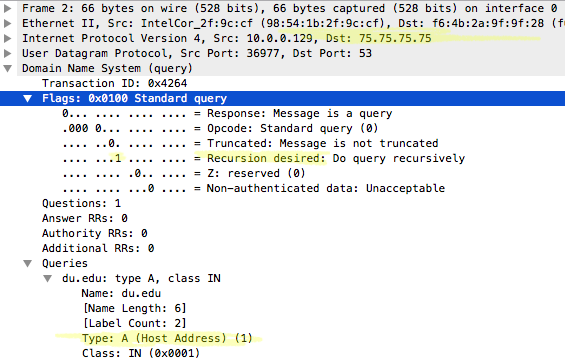
\includegraphics[height = 200pt, keepaspectratio]{Snapshots/q1/1_3_1.png}
\end{figure}
- The only flag set in the query is \textbf{recursion desired}.
\\
- To know the type of DNS server, we check the response to this query. 
\begin{figure}[H]
	\vspace{0pt}
	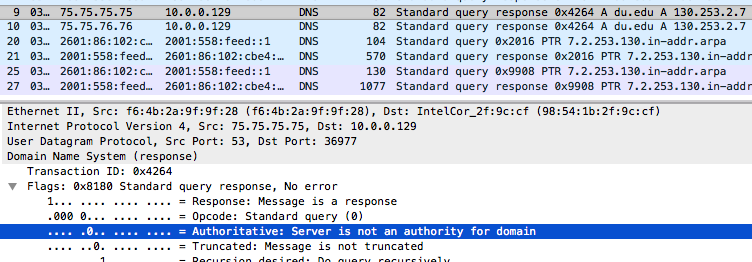
\includegraphics[height = 150pt, keepaspectratio]{Snapshots/q1/1_3_2.png}
\end{figure}
In the response, the flag \textbf{authoritative} is not set. Thus, it must be a local server having the IPA of the hostname cached. 

\subsection{:}

\begin{figure}[H]
	\vspace{0pt}
	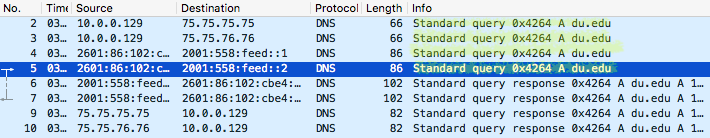
\includegraphics[height = 75pt, keepaspectratio]{Snapshots/q1/1_4.png}
\end{figure}
Total 4 DNS servers are queried for resolving the domain name du.edu.

\subsection{:}

\begin{figure}[H]
	\vspace{0pt}
	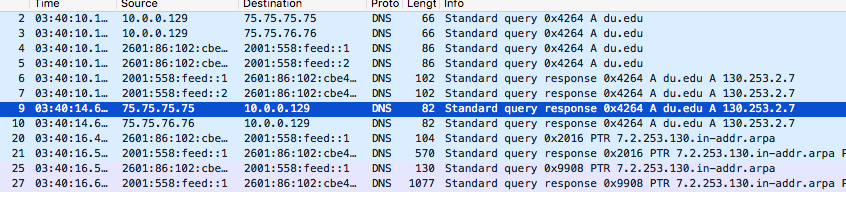
\includegraphics[height = 100pt, keepaspectratio]{Snapshots/q1/1_5_1.png}
\end{figure}

Packet \#9 contains the response of the query sent in packet \#2 as highlighted. The flags set are response, recursion desired and recursion available.

\begin{figure}[H]
	\vspace{0pt}
	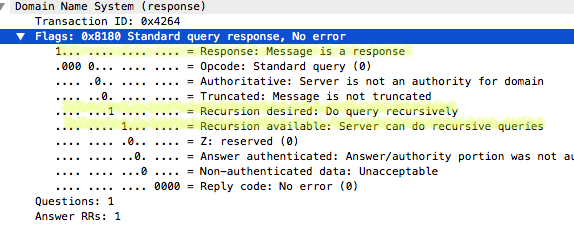
\includegraphics[height = 150pt, keepaspectratio]{Snapshots/q1/1_5_2.png}
\end{figure}

\subsection{:}

\begin{figure}[H]
	\vspace{0pt}
	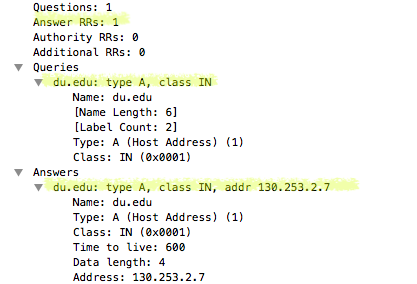
\includegraphics[height = 150pt, keepaspectratio]{Snapshots/q1/1_6_1.png}
\end{figure}

We get one answer from the server. The response is not from an authoritative server as this flag is not set. 

\begin{figure}[H]
	\vspace{0pt}
	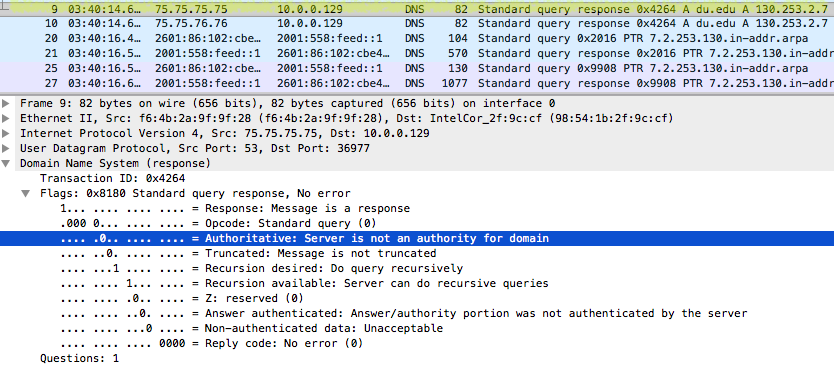
\includegraphics[height = 150pt, keepaspectratio]{Snapshots/q1/1_6_2.png}
\end{figure}

\subsection{:}

\begin{figure}[H]
	\vspace{0pt}
	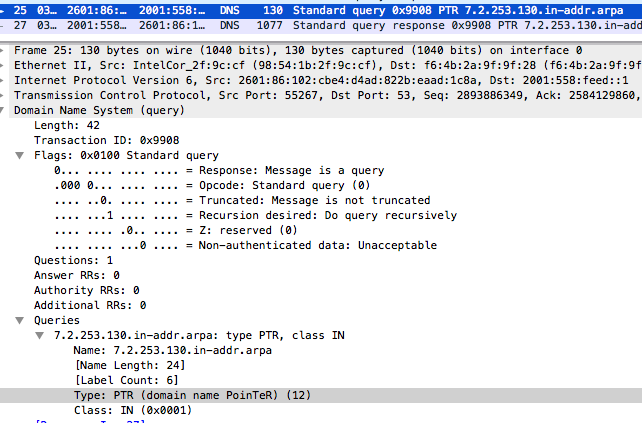
\includegraphics[height = 250pt, keepaspectratio]{Snapshots/q1/1_7.png}
\end{figure}

The query in packet \#25 is of the type PTR and it is used for reverse DNS lookup, i.e. given the IPA, the hostname is provided in the response. 

\subsection{:}

The packet \#27 contains the response of the packet \#25.
\begin{figure}[H]
	\vspace{0pt}
	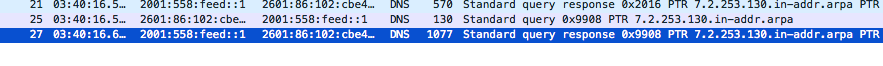
\includegraphics[height = 30pt, keepaspectratio]{Snapshots/q1/1_8_1.png}
\end{figure}

\begin{figure}[H]
	\vspace{0pt}
	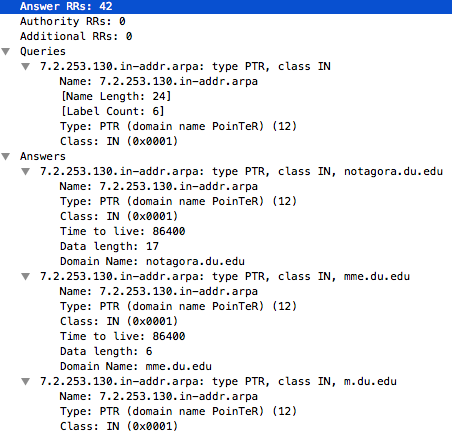
\includegraphics[height = 250pt, keepaspectratio]{Snapshots/q1/1_8_2.png}
\end{figure}
The response contains 42 resource records. All of them contain the hostname to which the queried IPA maps to. 

\section{SET 2: Using the DNS\_2.pcapng:}

\subsection{:}

\begin{figure}[H]
	\vspace{0pt}
	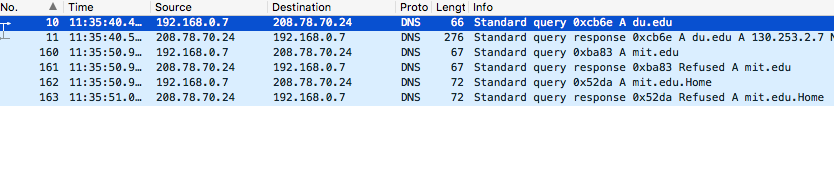
\includegraphics[height = 100pt, keepaspectratio]{Snapshots/q2/2_1_1.png}
\end{figure}

The destination IPA of the server is $208.78.70.24$. 

\begin{figure}[H]
	\vspace{0pt}
	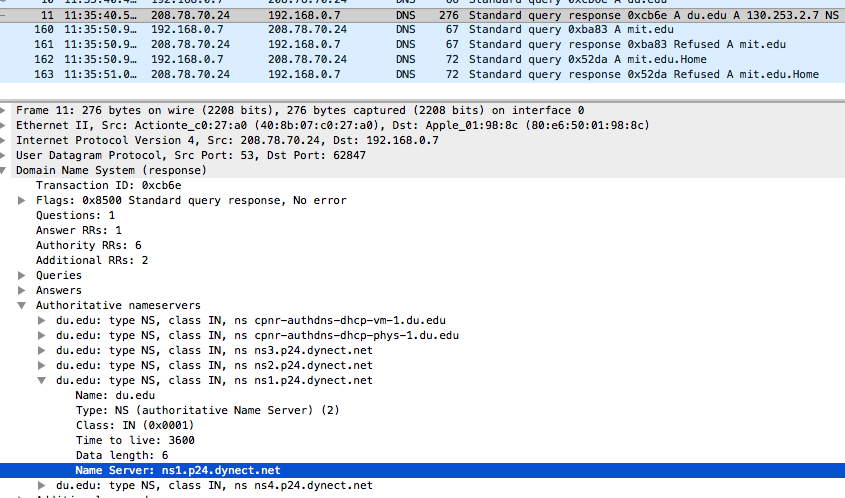
\includegraphics[height = 250pt, keepaspectratio]{Snapshots/q2/2_1_2.png}
\end{figure}

The request is being sent to the authoritative name server \textbf{ns1.p24.dynect.net} as seen in the response in the packet \#11. 

\subsection{:}

\begin{figure}[H]
	\vspace{0pt}
	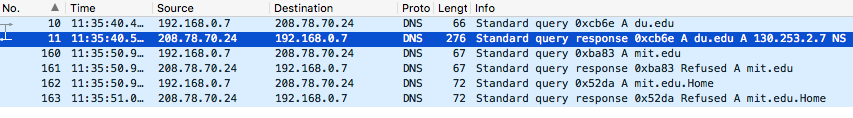
\includegraphics[height = 60pt, keepaspectratio]{Snapshots/q2/2_2_1.png}
\end{figure}

Packet \#11 contains the reply of the query sent in the packet \#10. Yes, the DNS server replied as we are getting a standard query response. 

\begin{figure}[H]
	\vspace{0pt}
	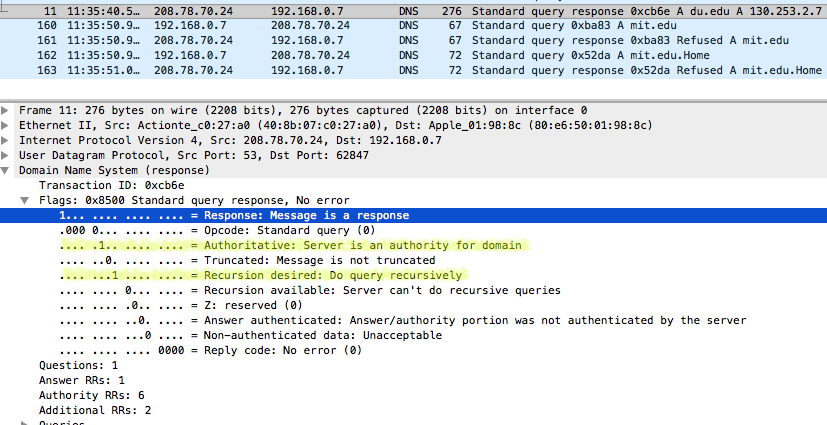
\includegraphics[height = 200pt, keepaspectratio]{Snapshots/q2/2_2_2.png}
\end{figure}

The response, recursion desired and authoritative flags are set in the response. 

\subsection{:}

\begin{figure}[H]
	\vspace{0pt}
	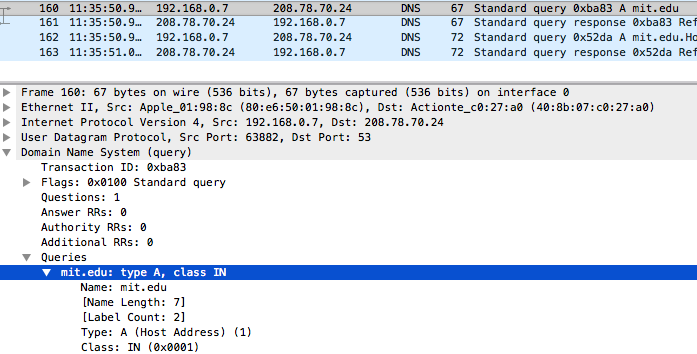
\includegraphics[height = 200pt, keepaspectratio]{Snapshots/q2/2_3.png}
\end{figure}

The DNS request in \#160 is sent to \textbf{ns1.p24.dynect.net}. The DNS request asks the IPA of the hostname \textbf{mit.edu} as the type of query is \textbf{A}.

\subsection{:}

The response from the DNS server for the query sent in packet \#160, as shown in the packet \#161, contains no answer RRs. The reply code is refused. So, the server did not resolve the DNS request. 

\begin{figure}[H]
	\vspace{0pt}
	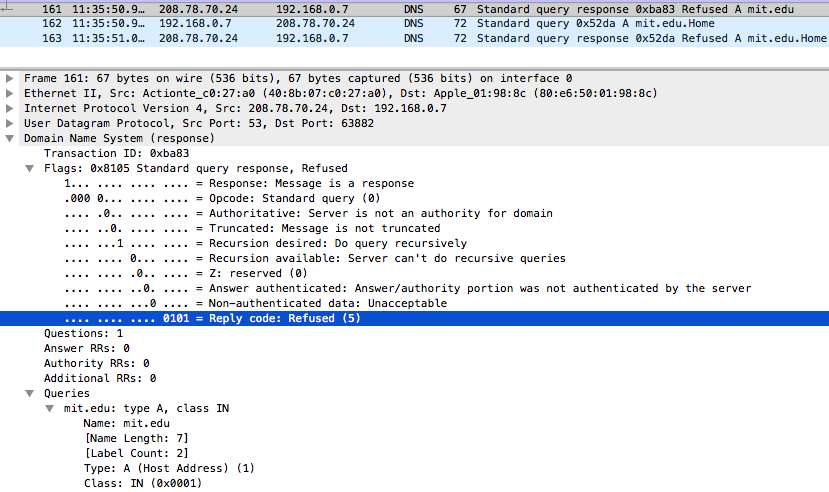
\includegraphics[height = 250pt, keepaspectratio]{Snapshots/q2/2_4.png}
\end{figure}

%%%%%%%%%%%%%%%%%%%%%%%%%%%%%%%%%%%%%%%%%%%%%%%%

\section{SET 3: Using the DNS\_3.pcapng:}

\subsection{:}
\begin{figure}[H]
	\vspace{0pt}
	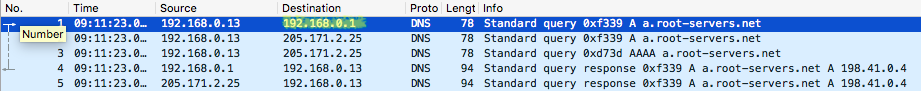
\includegraphics[height = 45pt, keepaspectratio]{Snapshots/q3/3_1.png}
\end{figure}
The DNS query in packet \#1 is sent to the IPA $192.168.0.1$. It is a local DNS server.

\subsection{:}
\begin{figure}[H]
	\vspace{0pt}
	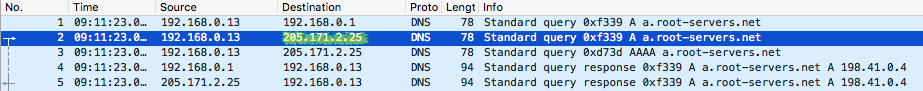
\includegraphics[height = 45pt, keepaspectratio]{Snapshots/q3/3_2.png}
\end{figure}
The DNS query in packet \#2 is sent to the IPA $205.171.2.25$. It is a local DNS server.


\subsection{:}
\begin{figure}[H]
	\vspace{0pt}
	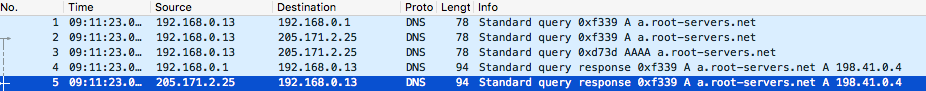
\includegraphics[height = 40pt, keepaspectratio]{Snapshots/q3/3_3_1.png}
\end{figure}

Packet \#5 contains the response of the packet sent in the query \#2.

\begin{figure}[H]
	\vspace{0pt}
	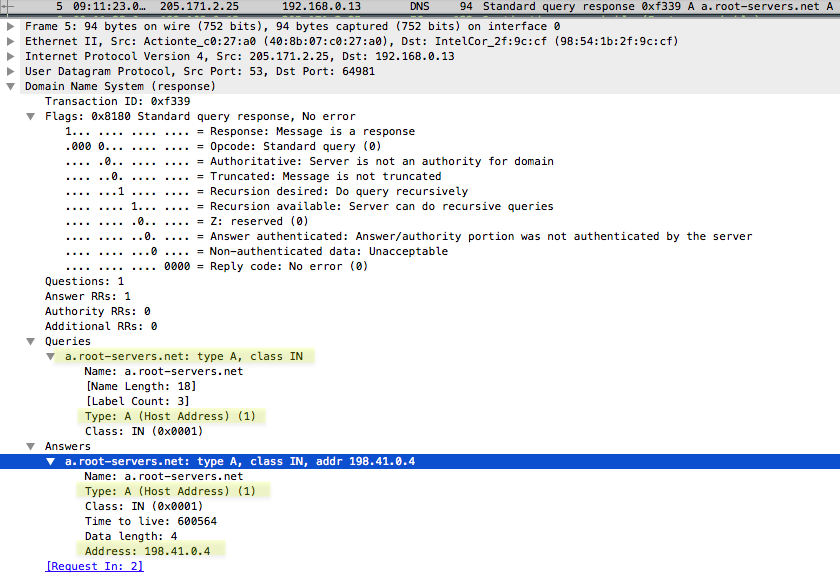
\includegraphics[height = 250pt, keepaspectratio]{Snapshots/q3/3_3_2.png}
\end{figure}

In the response, we get the IPA of the hostname \textbf{a.root-servers.net} which was what was queried as the type of query is \textbf{A}.

\subsection{:}
\begin{figure}[H]
	\vspace{0pt}
	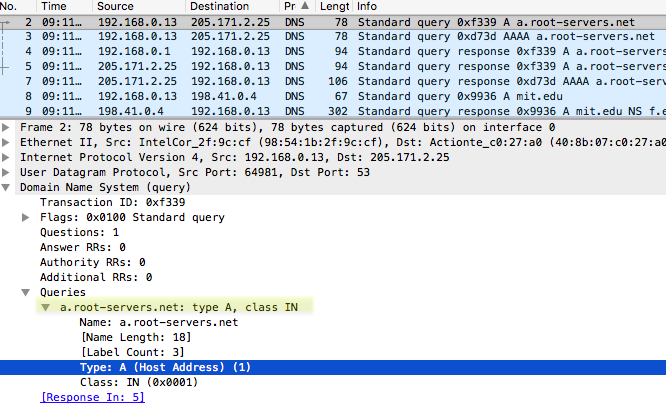
\includegraphics[height = 220pt, keepaspectratio]{Snapshots/q3/3_4_1.png}
\end{figure}

The difference between query in packet \#2 and packet \#3 is the type of the query. In \#2, query has type \textbf{A} which resolves the IPA in IPv4 whereas in \#3, query has type \textbf{AAAA} which resolves the IPA in IPv6. 

\begin{figure}[H]
	\vspace{0pt}
	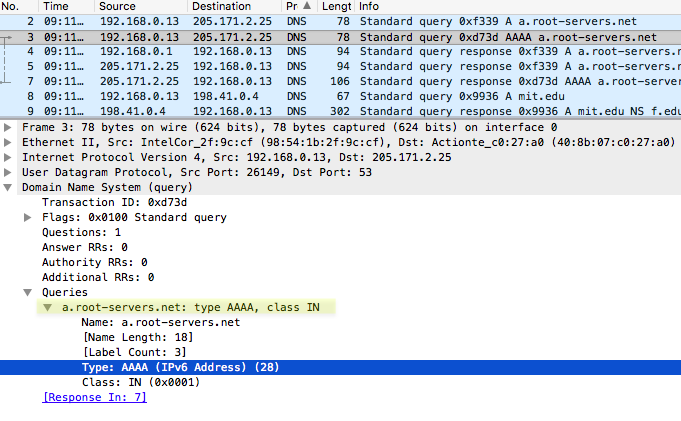
\includegraphics[height = 220pt, keepaspectratio]{Snapshots/q3/3_4_2.png}
\end{figure}

\subsection{:}
\begin{figure}[H]
	\vspace{0pt}
	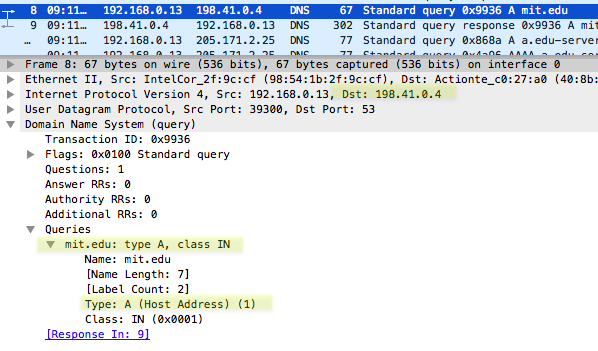
\includegraphics[height = 250pt, keepaspectratio]{Snapshots/q3/3_5.png}
\end{figure}
The query in packet \#8 is used to get the IPA of the hostname \textbf{mit.edu}  as the type of query is \textbf{A}. Since the IPA to which packet is sent is $198.41.0.4$ which was earlier resolved for the hostname \textbf{a.root-servers.net}, also the response in packet \#9 contains the list of .edu TLD servers, thus it is a \textbf{root server}.

\subsection{:}
\begin{figure}[H]
	\vspace{0pt}
	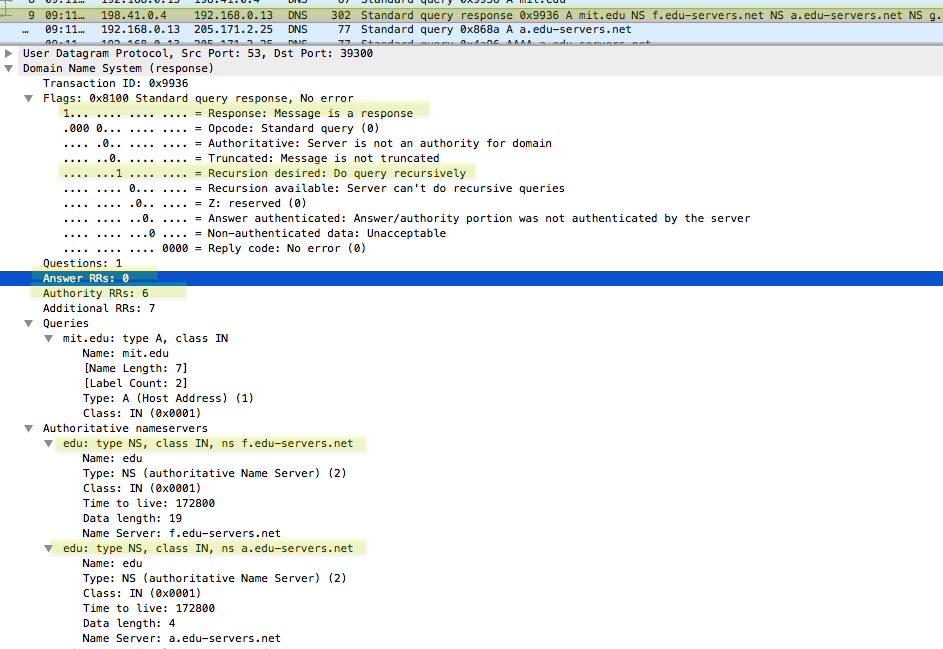
\includegraphics[height = 300pt, keepaspectratio]{Snapshots/q3/3_6.png}
\end{figure}

The packet \#9 contains the response of the query sent in packet \#8. The flags set in this are response and recursion desired. No, it does not have the answer the user wants as the no. of answer RRs = 0. It provides the list of .edu TLD servers. 
\subsection{:}
\begin{figure}[H]
	\vspace{0pt}
	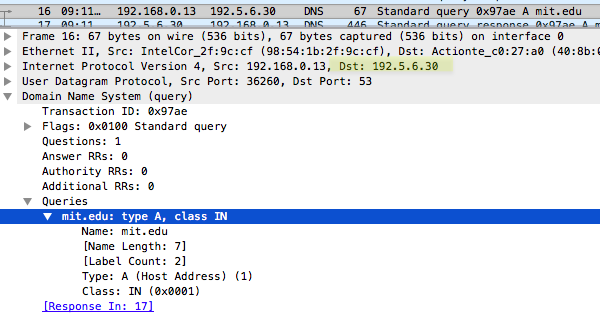
\includegraphics[height = 200pt, keepaspectratio]{Snapshots/q3/3_7.png}
\end{figure}

TLD server is being queried in the packet \#16. It is thus not a local DNS server. 

\subsection{:}
\begin{figure}[H]
	\vspace{0pt}
	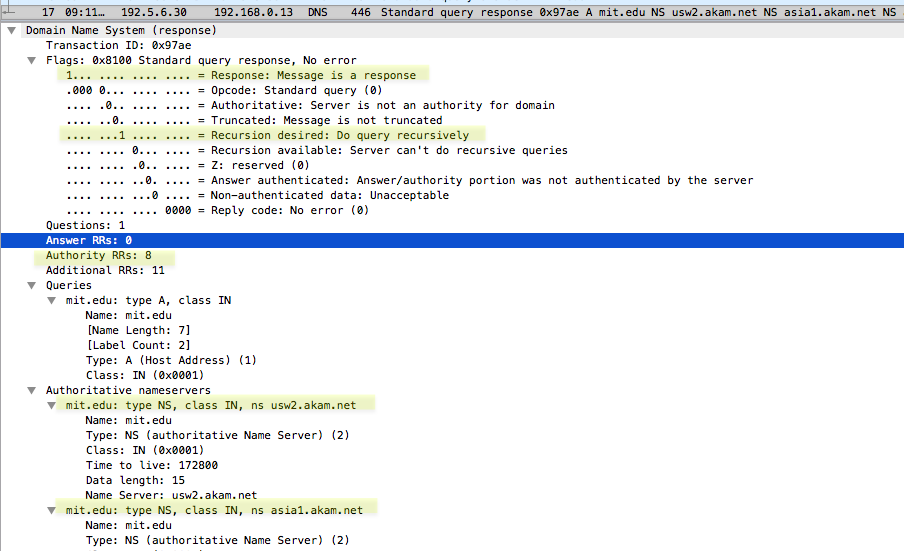
\includegraphics[height = 250pt, keepaspectratio]{Snapshots/q3/3_8.png}
\end{figure}
Packet \#17 contains the response of the query sent in the packet \#16. The flags set in this are response and recursion desired. No, it does not have the answer the user wants. It provides the information about the authoritative name servers as shown.

\subsection{:}
\begin{figure}[H]
	\vspace{0pt}
	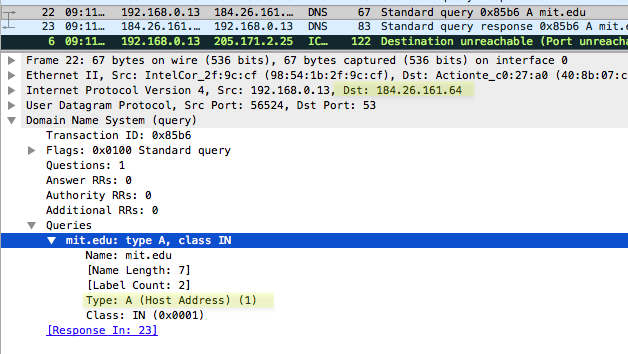
\includegraphics[height = 250pt, keepaspectratio]{Snapshots/q3/3_9.png}
\end{figure}

The query in packet \#22 is used to get the IPA of the hostname \textbf{mit.edu}  as the type of query is \textbf{A}. An authoritative name server is being queried. 

\subsection{:}
\begin{figure}[H]
	\vspace{0pt}
	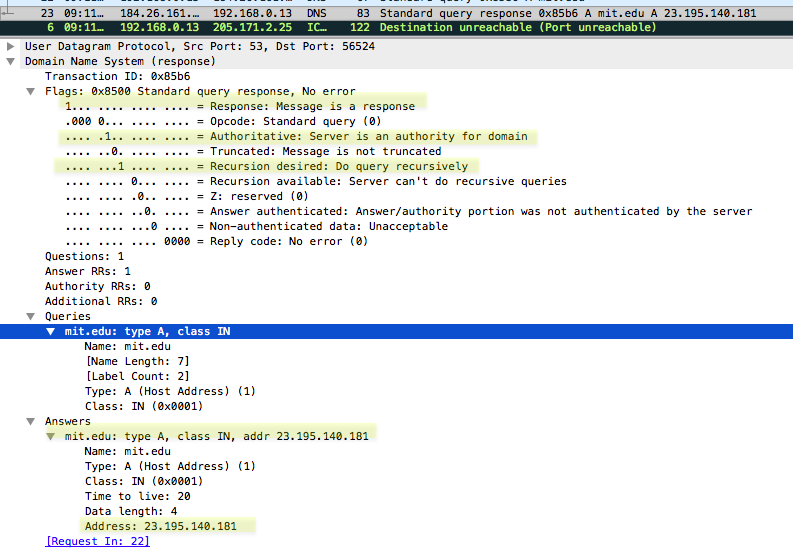
\includegraphics[height = 250pt, keepaspectratio]{Snapshots/q3/3_10.png}
\end{figure}

The packet \#23 contains the response of the packet \#22. The flags set in this are response, recursion desired and authoritative. Yes, it has the answer the user wants. It provides the IPA of the hostname \textbf{mit.edu}.

\section{Using dig command:}

\subsection{:}
\begin{figure}[H]
	\vspace{0pt}
	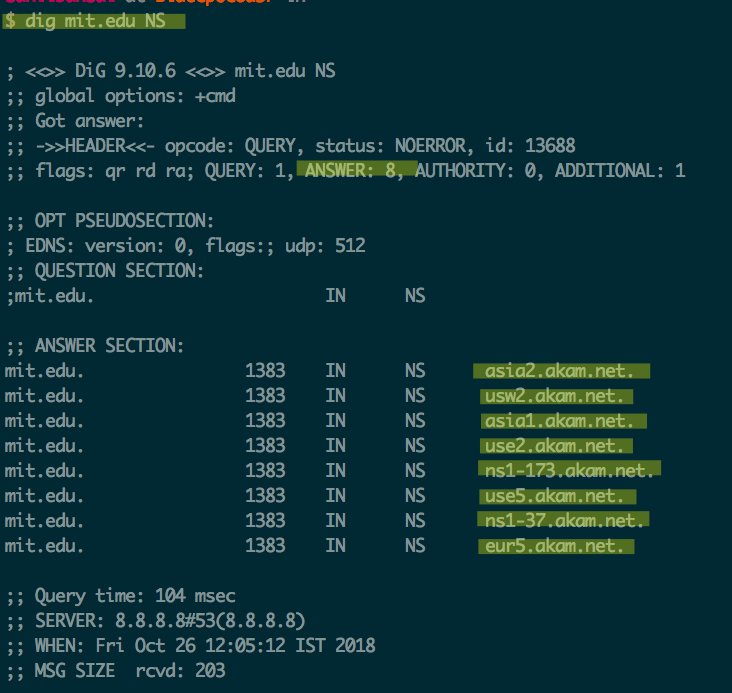
\includegraphics[height = 300pt, keepaspectratio]{Snapshots/q4/4_1.png}
\end{figure}
The dig command used to determine the authoritative DNS servers for \textit{mit.edu} is: \textbf{dig mit.edu NS} as highlighted. 

\subsection{:}
\begin{figure}[H]
	\vspace{0pt}
	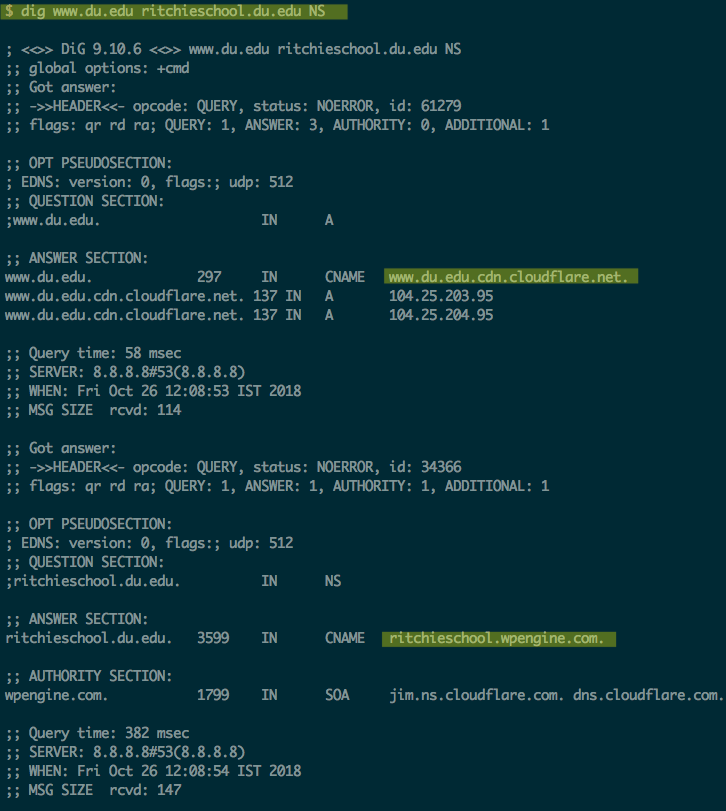
\includegraphics[height = 350pt, keepaspectratio]{Snapshots/q4/4_2.png}
\end{figure}
The command used to determine the authoritative DNS servers for \textit{www.du.edu} and \textit{ritchieschool.du.edu} in a single dig command is: \textbf{dig www.du.edu ritchieschool.du.edu NS}. \\

Since it does not provide any answer resource record of type NS, we run the command \textbf{dig +trace www.du.edu ritchieschool.du.edu} to see the complete execution of the DNS request. 
\begin{figure}[H]
	\vspace{0pt}
	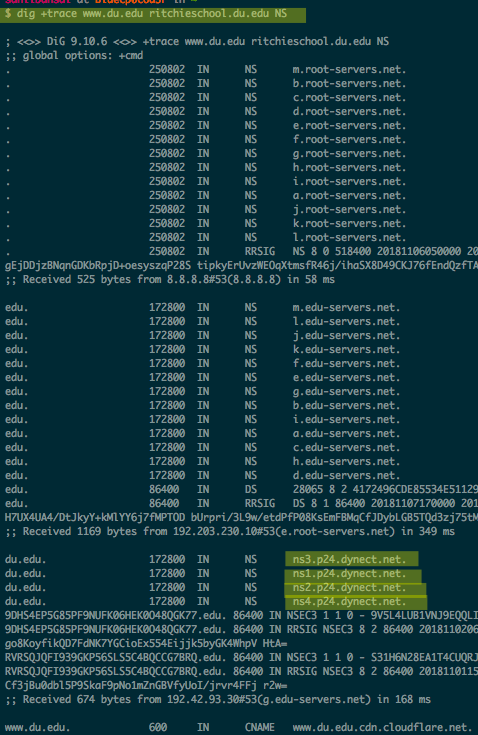
\includegraphics[height = 400pt, keepaspectratio]{Snapshots/q4/4_2_1.png}
\end{figure}

\begin{figure}[H]
	\vspace{0pt}
	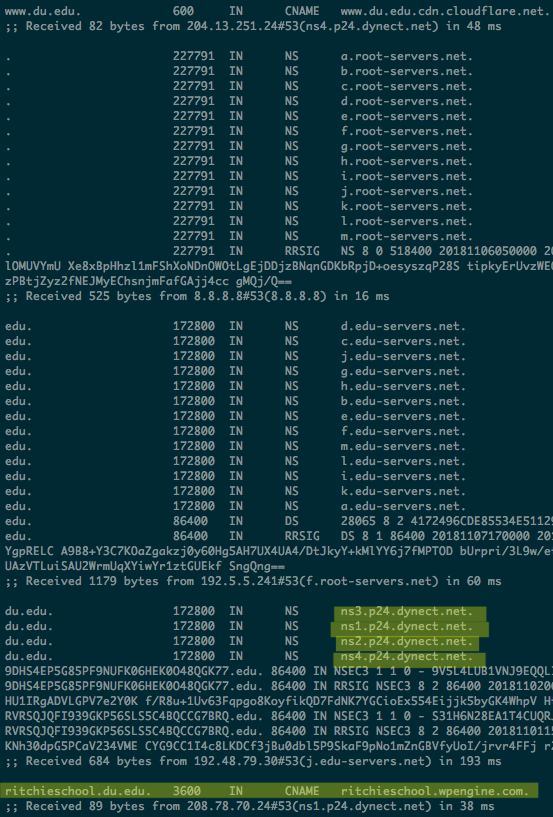
\includegraphics[height = 400pt, keepaspectratio]{Snapshots/q4/4_2_2.png}
\end{figure}

As we can see from this, the DNS servers are the same for both.
\subsection{:}
\begin{figure}[H]
	\vspace{0pt}
	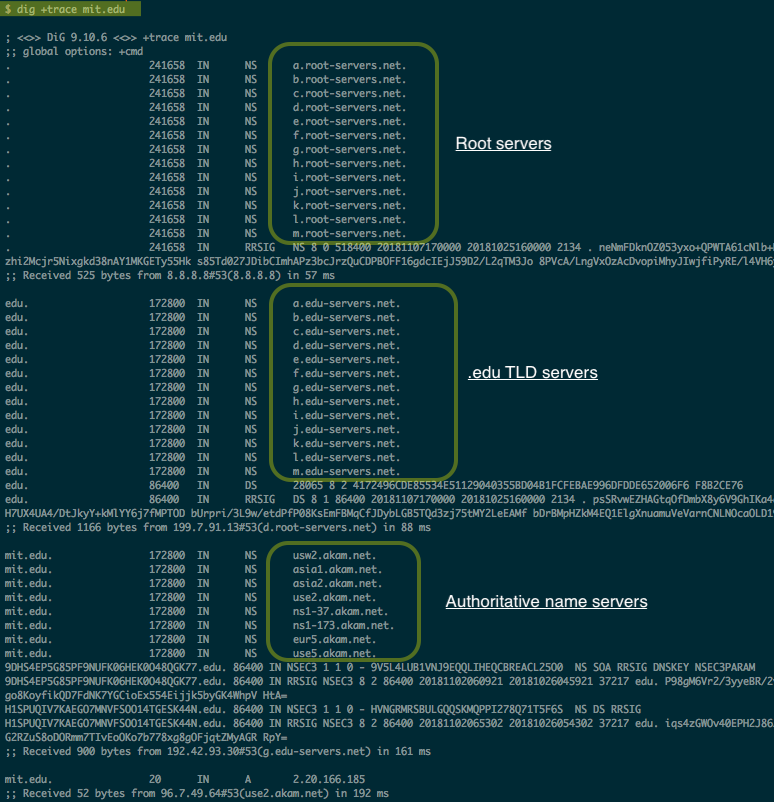
\includegraphics[height = 450pt, keepaspectratio]{Snapshots/q4/4_3.png}
\end{figure}
We can infer from this output that the DNS request first goes to the root servers, then it goes to the .edu TLD servers and then finally the authoritative name servers for mit.edu. 

\end{document}